\chapter{Choix d'implémentation}

\section{Fonctionnement général}

\paragraph{}L'utilisateur fourni un fichier et précise son type. Il peut aussi choisir d'afficher des labels sur les n\oe uds ainsi que le format de sortie souhaité. Par défaut, l'application génère un png sans labels. L'application fonctionne ensuite en trois étapes:
\begin{enumerate}
	\item Parsing du fichier d'entrée selon le type indiqué pour obtenir une représentation d'arbre selon notre structure interne.
	\item Calcul des coordonnées de chaque n\oe ud.
	\item Génération d'une image selon le type de sortie choisie.
\end{enumerate}

\begin{center}
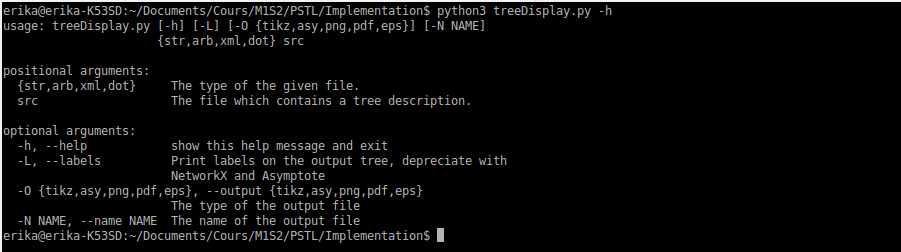
\includegraphics[width=\columnwidth]{usage}
\end{center}

\section{Plus en détails}

	\subsection{Structure d'arbre}
	
\lstinputlisting[language=Python, firstline=4, lastline=17]{../Src/tree.py}

	\subsection{Fonctionnement des algorithmes de parsing}

\paragraph{Mots bien parenthésés}Le parser de mots bien parenthésés (cf. \ref{dotParser}) respecte la grammaire suivante:
		
\begin{verbatim}
ARBRE : '(' ID NOEUDS ')'
NOEUDS : ARBRE NOEUDS | e
ID : [a-zA-Z1-9]* | e
\end{verbatim}
		
\paragraph{Dot}Le parser dot parse une sous-partie du langage dot, à savoir:

\begin{verbatim}
DOT : STRICT GRAPH ID '{' SEQINST '}'
STRICT : strict | e
GRAPH = diagraph | graph
SEQINST : INST SEQINST | e
INST : REF [label = "ID"] ';' | REF LINK REF
LINK : -- | ->
REF : [0-9]*
ID : [a-zA-Z1-9]* | e
\end{verbatim}
		
\paragraph{XML}Le parser XML utilise la librairie XML de Python. Il respecte la grammaire suivante:
		
\begin{verbatim}
XML : <?xml version="1.0"?><tree> NOEUDS <tree>
NOEUDS : NOEUD NOEUDS | e
NOEUD : <node type=TAG id=ID> NOEUDS </noeud> | <leaf type=TAG id=ID />
TAG : "Leaf" | "BinNode"
\end{verbatim}

	\subsection{Fonctionnement de l'algorithme de calcul de coordonnées}

\paragraph{}On décide que la distance minimale entre deux n\oe uds est de $1$ unité.

\paragraph{}L'ordonnée d'un n\oe ud est triviale: c'est sa profondeur.

\paragraph{}L'abcisse d'un n\oe ud est un peu plus complexe et demande donc plus de réflexion. Pour un n\oe ud donné, on commence par placer ses fils. On centre ensuite ce n\oe ud au milieu de ses fils en faisant la moyenne de l'absisse de ses deux fils extrémaux. Si un n\oe ud n'a pas de fils, on le place à $1$ de son frère gauche. D'un point de vue de l'architecture, on a donc besoin d'une structure qui, à profondeur \emph{p} mémorise la prochaine place disponible (ou au choix la dernière place utilisée.\\
Si un père a des fils, on le centre au milieu de ses fils. Par ce calcul, on peut se retrouver avec un n\oe ud qui est trop proche de son frère gauche [Mettre un exemple]. Pour cela, on compare la position calculée avec la première position disponible et on prend le max. Si la position calculée n'est pas celle retenue, le père n'est plus centré au milieu de ses fils. On mémorise donc le décalage effectué pour ce père pour ensuite l'appliquer à ses sous-arbre dans un second temps.
\begin{enumerate}
	\item Pour un n\oe ud donné, on commence par placer ses fils.
	\item On centre ensuite ce n\oe ud au milieu de ses fils.
	\item Si un n\oe ud collisionne avec son frère gauche, on le décale vers la droite et on mémorise ce décalage car il faudra ensuite décaler ses sous-arbres. On applique ce décalage dans une seconde passe pour des raisons de complexité. En effet, si on faisait chaque décalage lorsqu'il se présentait, le décalage serait quadratique alors que dans le cas choisi, on est linéaire.
\end{enumerate}

	\subsection{Fonctionnement de la génération du code}
	
\paragraph{TikZ}
		
\paragraph{Asymptote}
		
\paragraph{Autre}

\section{Complexité}

\paragraph{}On suppose que la taille des labels est bornée. On note $n$ le nombre de n\oe uds dans l'arbre. Dans ce cas:

\begin{enumerate}
	\item Le parsing d'un fichier est en $O(n)$.
	\item Le calcul des coordonnées est en $O(n)$ (on effectue $2$ passes sur l'arbre).
	\item La génération du fichier de sortie est en $O(n)$.
\end{enumerate}
On a donc une complexité générale en $O(n)$ où $n$ est le nombre de n\oe ud de l'arbre.

\paragraph{}Notons que nous avons supposé que la taille des labels était bornée. Or nous n'avons aucune prise sur la taille des labels du fichier qui nous est passé en entrée. Dans ce cas, même si on borne la taille des labels pour l'affichage, la complexité est dominée par le parsing du fichier d'entrée car on doit lire tous les caractères du fichier.